\section{Evaluation for Faraday effect}
Now we fitted the plots with a leastsquare linear polynomial:
\begin{equation}
    \alpha(I) = p_1 I + p_1
\end{equation}
As it turns out the given standard deviations seem to be estimated much to high,
one would expect more fluctuation 
around the fitted polynome. This observation can be made more 
precise using the $\chi^2$-test. For a variable $y_i$ in a sample of 
size $N$ assumed to follow 
a gaussian disribution around its expectation value, which in case of 
an underlying functional relation to another variable $x_i$ is assumed 
to be $\lambda(x_i; \theta)$, where $\theta$ are the parameters of 
the fit, we can define the quantity
\begin{equation}
    \chi^2(\theta) = \sum_{i, j= 1}^N (y_i - \lambda(x_i; \theta))
        (V^{-1}) (y_j - \lambda(x_j; \theta)), 
\end{equation}
where $V^{-1}$ is the inverse of the covariance matrix $\mathrm{cov}(i,j)$. 
The least square fit is done by simply minimizing the quantity. If the 
variables do follow the suspected functional relation and are distributed 
with a variance $\sigma_i^2$, then $\chi^2$ should follow the 
$\chi^2$-distribution with expectation value $n_d$, where $n_d$ is 
the number of points minus the number of paramter $\theta$.
One can thus test the applied hypothesis by calculating $\chi^2$ and 
dividing it by $n_d$, getting a numerical value for the 
\emph{godness-of-fit}. Pursuing the goal of the experiment we now turn to the 
calculation of the \textit{Verdet} constant. As we calculated the covariance matrix from the
plots, we will use measurement \textbf{2.4} for the further calculations. Since we used
a randomized array of Currents we tried to minimize the systematic error which resulted
in the most stable behavior of the measurements.

\begin{eqnarray}
    \mathrm{cov}(p_i, p_j) &=& 
    \begin{pmatrix}
        1.443\mathrm{e}-04 &-3.391\mathrm{e}-04 \\
        -3.391\mathrm{e}-04 &1.014\mathrm{e}-03 \\
    \end{pmatrix}
\\ \Rightarrow \qquad
    p_1 &=& 2.606 \pm 0.012 \cm\\
    p_2 &=& 0.349 \pm 0.032 \cm \\
    \chi ^2/(N-1) &=&  0.124
\end{eqnarray}
The displacement $p1$ can be explained in terms of the experimental setup: The Gauge of the 
angle is not fixed such that the lower limit is zero. Since we are only interested in the slope,
this is not relevant for the result. The $\chi^2$-test is too low, which either indicates that
the functional relationship between the variables is fulfilled very poorly or that the chosen
standard deviation is estimated to high. The latter is not unprobable, since it is also
visible optically, see figure~\ref{fig:23}. Now we turn our attention to the calculation:
\begin{align}
    V &= \frac{\alpha}{I\mu}   = p_2 / \mu \\
      &= \left [ 1.019 \pm 0.005 \right ]\cdot 10^{-3} \quad \mathrm{Deg/A} \\
      &= \left [ 0.04868 \pm 0.00022 \right ] \cdot 10^{-3} \quad \mathrm{Deg/A}
\end{align}
Where we use $1\ \mathrm{Oe} = \frac{1000}{4\pi}\ \mathrm{A/m}$, $\quad1$ Deg $=60$ min \quad and $\mu = 2556$.




\begin{figure}
    \begin{centering}
        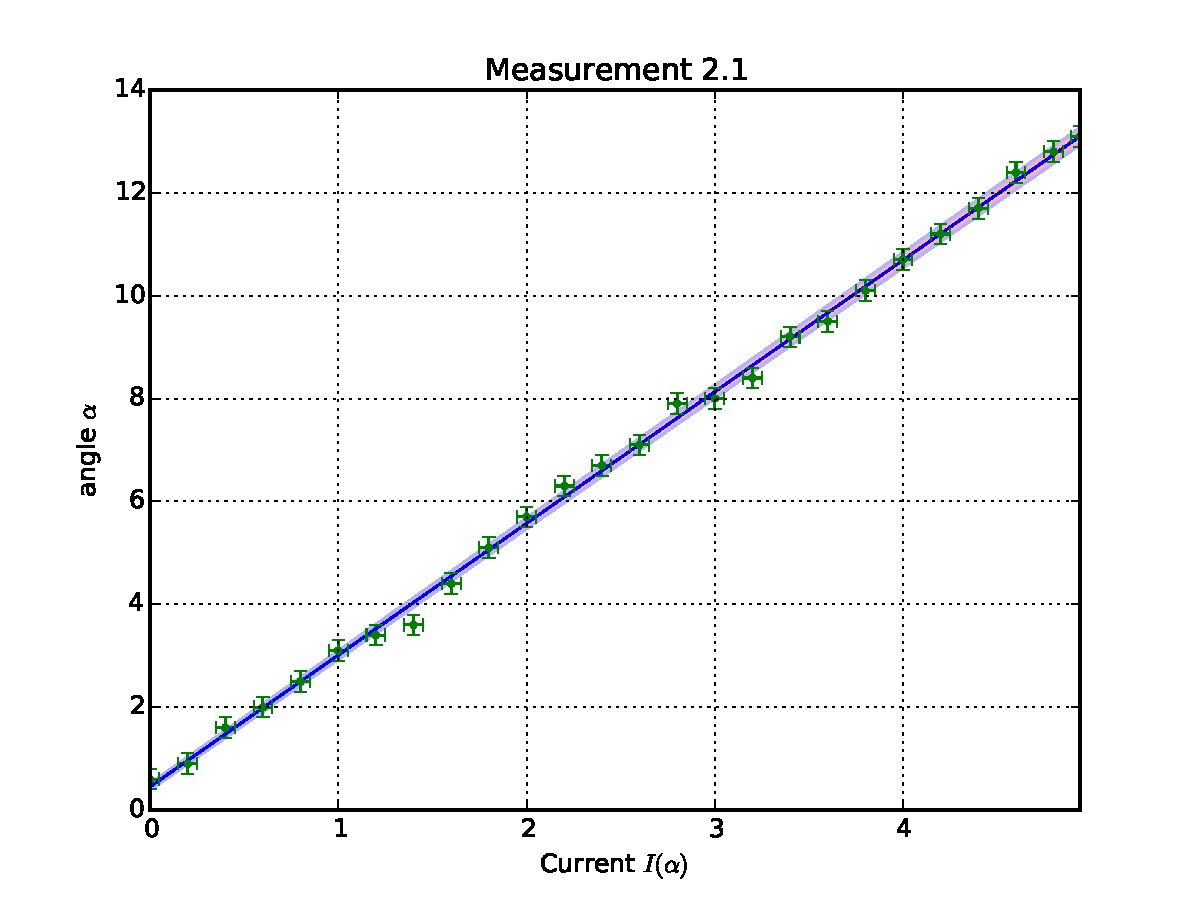
\includegraphics[width=18cm]{figures/fig21}
\captionsetup{singlelinecheck=off} 
\caption[.]{
\begin{eqnarray*}
    \mathrm{cov}(p_i, p_j) &=& 
    \begin{pmatrix}
        4.511\mathrm{e}-04 &-1.127\mathrm{e}-03 \\
        -1.127\mathrm{e}-03 &3.824\mathrm{e}-03 \\
    \end{pmatrix}
\\ \Rightarrow \qquad
    p_1 &=& 2.561 \pm 0.021 \cm\\
    p_2 &=& 0.45 \pm 0.06 \cm \\ 
    \chi ^2/(N-1) &=&  0.577
\end{eqnarray*}
}

    \end{centering}
\end{figure}
\begin{figure}
    \begin{centering}
        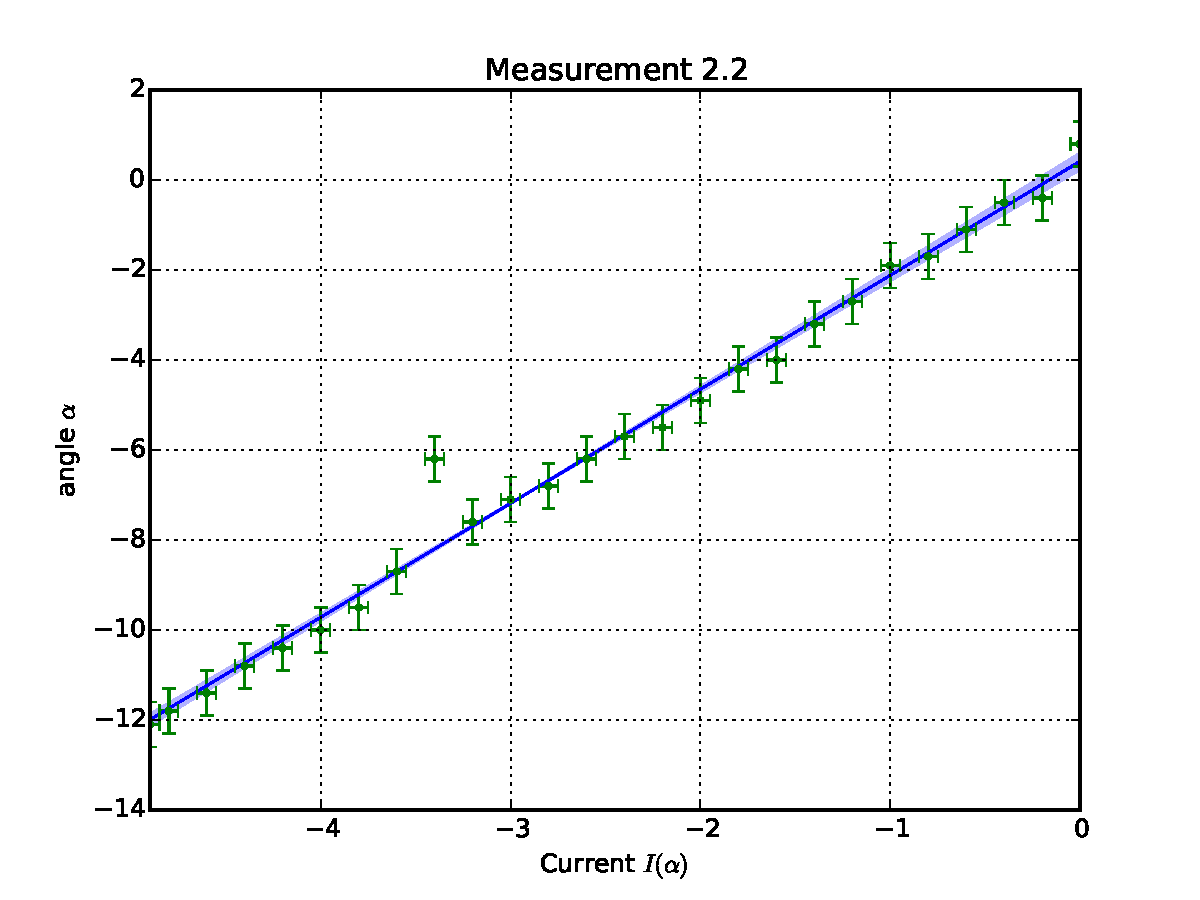
\includegraphics[width=18cm]{figures/fig22}
\captionsetup{singlelinecheck=off} 
\caption[.]{
\begin{eqnarray*}
    \mathrm{cov}(p_i, p_j) &=& 
    \begin{pmatrix}
        3.835\mathrm{e}-03 &9.572\mathrm{e}-03 \\
        9.572\mathrm{e}-03 &3.245\mathrm{e}-02 \\
    \end{pmatrix}
\\ \Rightarrow \qquad
    p_1 &=& 2.53 \pm 0.06 \cm\\
    p_2 &=& 0.41 \pm 0.18 \cm \\
    \chi ^2/(N-1) &=& 0.715
\end{eqnarray*}
}



%\label{fig:fig22}
    \end{centering}
\end{figure}

\begin{figure}
    \begin{centering}
        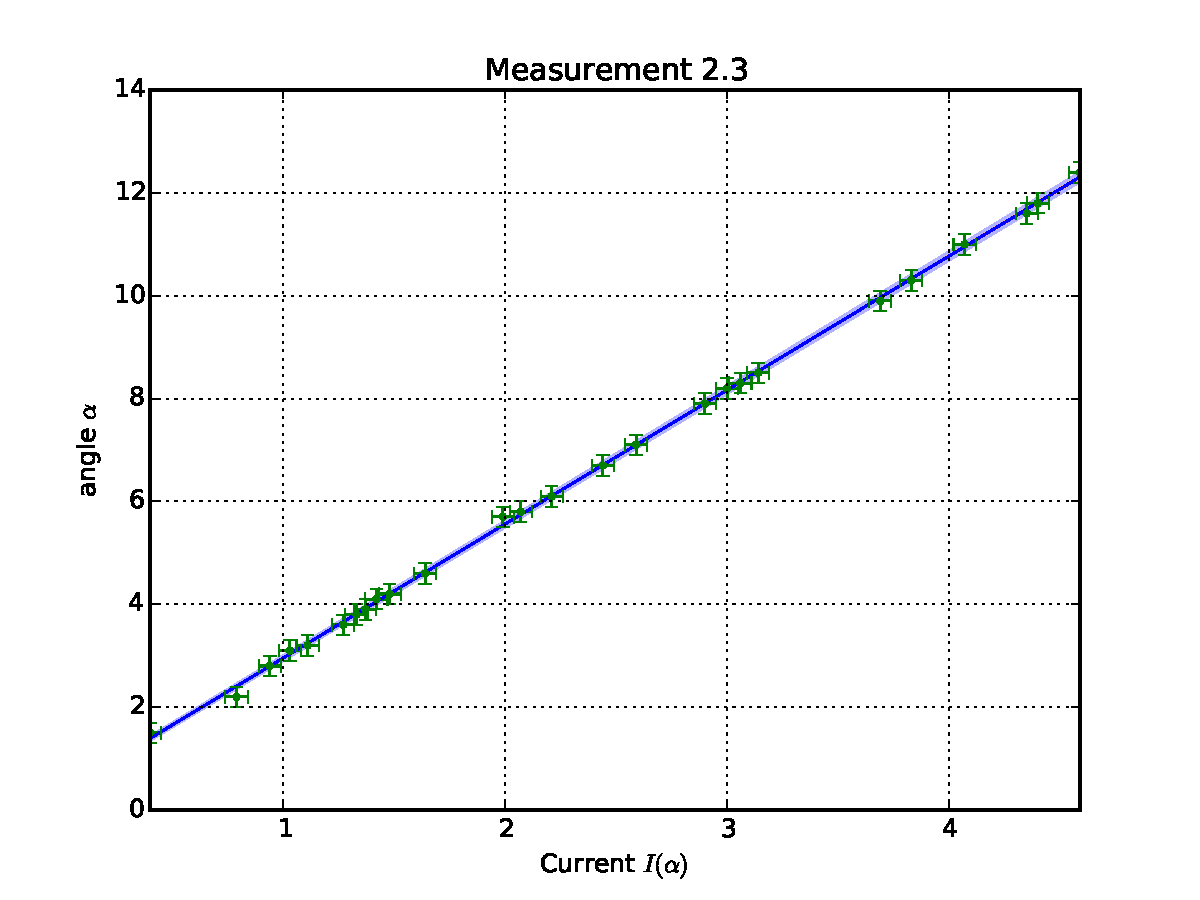
\includegraphics[width=18cm]{figures/fig23}
\captionsetup{singlelinecheck=off} 
\caption[.]{
\begin{eqnarray*}
    \mathrm{cov}(p_i, p_j) &=& 
    \begin{pmatrix}
        1.443\mathrm{e}-04 &-3.391\mathrm{e}-04 \\
        -3.391\mathrm{e}-04 &1.014\mathrm{e}-03 \\
    \end{pmatrix}
\\ \Rightarrow \qquad
    p_1 &=& 2.606 \pm 0.012 \cm\\
    p_2 &=& 0.349 \pm 0.032 \cm \\
    \chi ^2/(N-1) &=&  0.124
\end{eqnarray*}
}
\label{fig:23}
    \end{centering}
\end{figure}


\begin{figure}
    \begin{centering}
        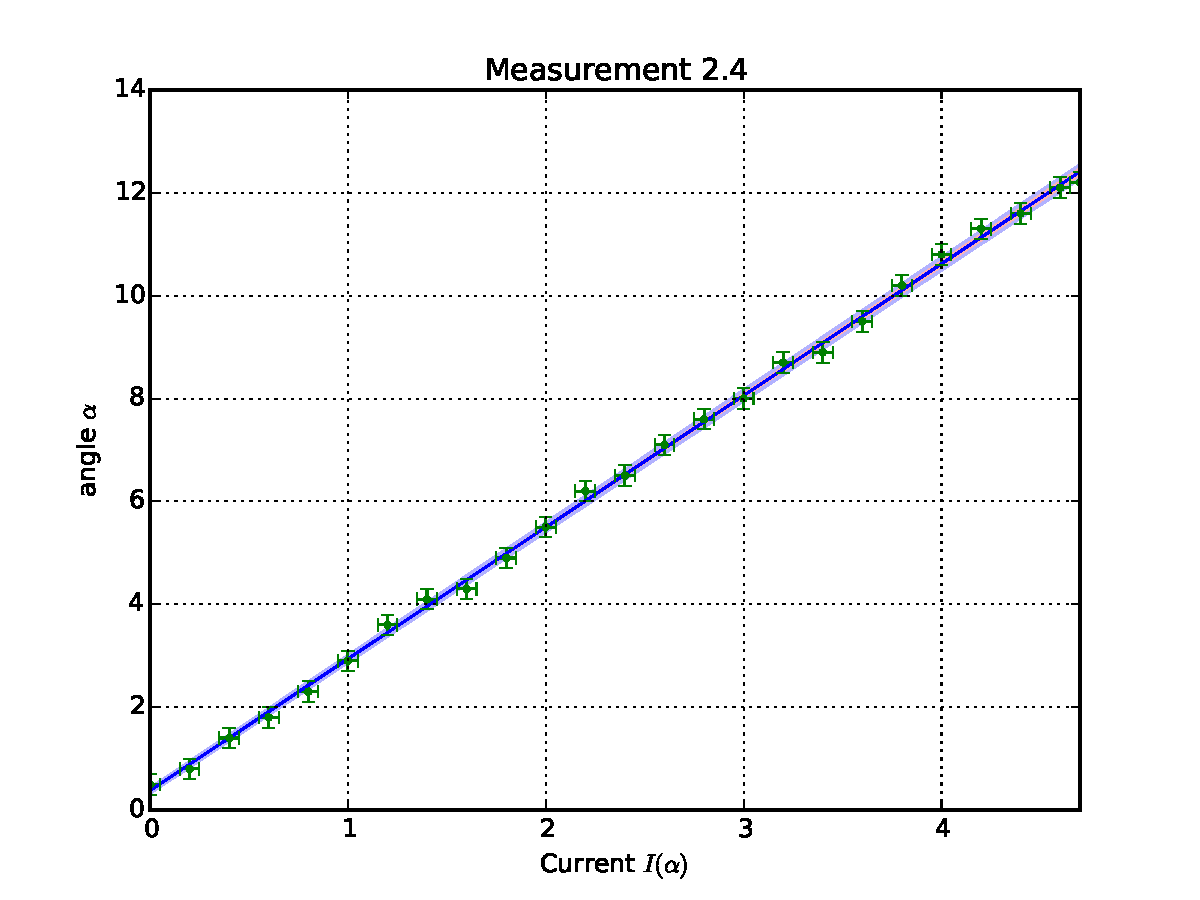
\includegraphics[width=18cm]{figures/fig24}
\captionsetup{singlelinecheck=off} 
\caption[.]{
\begin{eqnarray*}
    \mathrm{cov}(p_i, p_j) &=& 
    \begin{pmatrix}
        3.310\mathrm{e}-04 &-7.931\mathrm{e}-04 \\
        -7.931\mathrm{e}-04 &2.582\mathrm{e}-03 \\
    \end{pmatrix}
\\ \Rightarrow \qquad
    p_1 &=& 2.561 \pm 0.018 \cm\\
    p_2 &=& 0.38 \pm 0.05 \cm \\
    \chi ^2/(N-1) &=&  0.373
\end{eqnarray*}
}
    \end{centering}
\end{figure}


